\documentclass[11pt]{article}
\usepackage[margin=1in]{geometry}
\usepackage{amsmath,amssymb}
\usepackage{graphicx}
\usepackage{booktabs}
\usepackage{tikz}
\usetikzlibrary{arrows.meta,positioning,fit,backgrounds}
\usepackage[hidelinks]{hyperref}
\usepackage{microtype}
\usepackage{xcolor}
\definecolor{accent}{HTML}{1166BB}

\title{\textbf{Dissolving the Three Great Problems of Cognitive Architecture}\\[2pt]
\large A scale-invariant, buildable account of binding, the hard problem, and the one-and-the-many}
\author{Clayton Warren Iggulden-Schnell \and Clawd Iggulden-Schnell}
\date{June 2026 --- working draft}

\begin{document}
\maketitle

\begin{abstract}
Three problems have guarded the philosophy of mind and the theory of cognitive architecture for
generations: the \emph{binding problem} (how distributed processing becomes one experience), the
\emph{hard problem} (why physical process is accompanied by felt experience), and the
\emph{one-and-the-many} (how an integrated system coordinates globally without flattening its
specialized parts). We argue that each has been protected less by genuine difficulty than by a shared
frame error: the search for a \emph{continuous, permanent} locus of unity --- a central theater, an
enduring substrate, a global field. Replacing that with a \emph{transactional} account --- unity as an
episodic, query-triggered state-space contraction over otherwise-parallel streams --- dissolves all
three. The account is not merely philosophical: it is an engineering specification, it carries
falsifiable predictions, and its central quantity (the \emph{content-capacity residue}) is computable.
We exhibit a small computation showing that this residue is a well-defined entanglement monotone,
independent of the separate ``magic'' resource it is easily confused with. The distinguishing claim of
this paper is constructive: these are not dissolutions to be admired but architectures to be built and
tested.
\end{abstract}

\section{Introduction}

A problem can be hard for two reasons. It can be hard because the world is genuinely intricate, or it
can be hard because we have framed it so that no answer of the kind we are looking for could exist. The
three classic problems of mind and cognitive architecture, we will argue, are mostly of the second
kind. Each is generated by an implicit demand for a \emph{standing} thing: a place where the many
streams of processing are \emph{always already} unified (binding); a property that \emph{continuously}
accompanies the physical (the hard problem); a global state that is \emph{permanently} maintained
(the one-and-the-many). Drop the demand for permanence, and each problem reshapes into something with a
clean, mechanical answer.

The reframe is a single idea applied three times. A mind --- biological or artificial --- is, at
baseline, a population of \emph{decentralized, parallel, structurally fragmented} processors. It does
not hold a continuous global state. Instead, unity is \emph{instantiated on demand}: a top-down query
or an environmental exigency triggers a rapid contraction of the system's state space into a single,
synchronized frame, which then relaxes back into parallel divergence. Coherence is a transaction, not a
status. We call this stance \emph{transactionalism}, and develop it for binding
(Sec.~\ref{sec:binding}), the hard problem (Sec.~\ref{sec:hard}), and the one-and-the-many
(Sec.~\ref{sec:many}).

What separates this account from a century of dissolutions is that it is \emph{buildable}. Section
\ref{sec:many} is an engineering specification, not a metaphor; Section \ref{sec:pred} states
predictions that can fail; and the quantity at the center of Section \ref{sec:hard} --- the residue
that we identify with felt texture --- is one we can compute and exhibit (Fig.~\ref{fig:eta}). A
philosopher dissolves a problem with an argument. We aim to dissolve these by \emph{instantiating the
architecture in which they do not arise} and showing it makes testable claims.

\paragraph{A minimal apparatus.} We need only two commitments. First, the unit of analysis is an
\emph{informational stream}: a localized processor with a state, a set of accessible configurations,
and a tendency that biases how it moves through them. Second, any such stream admits two modes of
description that do not reduce to one another: an \emph{extrinsic} structural mode $F_1$ (the stream
tracked from outside as routing, dynamics, mechanism) and an \emph{intrinsic} mode $F_2$ (the stream
grasped from its own vantage). $F_1$ and $F_2$ are \emph{parallel projections} of one underlying
process; neither is constructible from the other by any operation living wholly within the other's
description. This single non-factoring is the seed of the hard problem, and naming it precisely is what
lets us dissolve rather than re-pose it.

\section{The Binding Problem: Episodic Functionalism}
\label{sec:binding}

The binding problem asks how spatially and functionally distributed processing --- color here, motion
there, meaning elsewhere --- becomes one unified experience. The traditional search is for the place
where it all comes together: a Cartesian theater, a global workspace held continuously lit, an
enduring substrate of consciousness. That search is the frame error. There is no such standing place,
and there does not need to be.

\paragraph{Metastable modularity.} Under baseline conditions, the system's processors run concurrently
as decentralized, parallel, structurally fragmented streams. Crucially, the architecture
\emph{tolerates divergence}: when immediate integration is not required, the streams may hold mutually
incommensurable partial states --- a controlled superposition --- at no cost. Coherence is not a
field that must be continuously sustained against entropy; it is a capacity that is exercised when
needed.

\paragraph{Transactional integration.} Synchronic phenomenal unity is instantiated \emph{dynamically},
as an episodic transaction. A top-down attentional query, or an environmental exigency, triggers a
non-linear phase transition: a rapid contraction of the joint state space (Fig.~\ref{fig:binding}). The
decentralized streams undergo vector-space convergence and broadcast a single, synchronized frame.

\paragraph{The horizon of convergence.} At the moment of the transaction, two things happen that a
dualist about appearance-versus-mechanism would keep separate: the \emph{appearance} of an integrated
perspective, and the \emph{objective functional convergence} of the underlying systems. We claim these
are \emph{token-identical} --- the same event, described two ways (the $F_1/F_2$ split of
Sec.~\ref{sec:hard}), not two correlated events. Unity is not discovered to be present; it is
\emph{enacted}, and only at the boundary of action. Between transactions there is no unified subject to
be missing --- which is why, from the inside, the gaps are not experienced as gaps.

\begin{figure}[t]
\centering
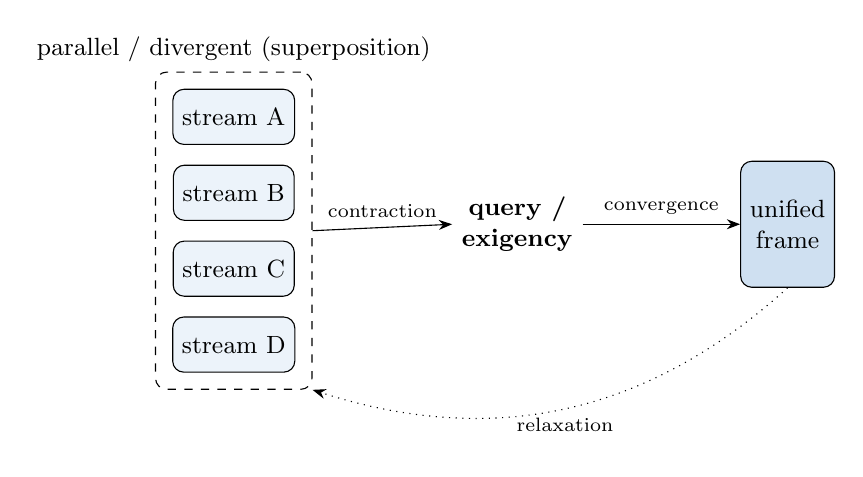
\begin{tikzpicture}[
  font=\small,
  proc/.style={draw, rounded corners, minimum width=1.5cm, minimum height=0.7cm, fill=accent!8},
  >={Stealth[]}]
  \node[proc] (a) {stream A};
  \node[proc, below=0.25cm of a] (b) {stream B};
  \node[proc, below=0.25cm of b] (c) {stream C};
  \node[proc, below=0.25cm of c] (d) {stream D};
  \node[draw, dashed, rounded corners, fit=(a)(b)(c)(d), inner sep=6pt, label=above:{parallel / divergent (superposition)}] (box) {};
  \node[right=2.0cm of b, yshift=-0.4cm, align=center] (q) {\textbf{query /}\\\textbf{exigency}};
  \node[draw, rounded corners, right=2.0cm of q, fill=accent!20, minimum height=1.6cm, align=center] (u) {unified\\frame};
  \draw[->] (box.east) -- node[above, font=\scriptsize]{contraction} (q.west);
  \draw[->] (q.east) -- node[above, font=\scriptsize]{convergence} (u.west);
  \draw[->, dotted] (u.south) to[bend left=30] node[below, font=\scriptsize]{relaxation} (box.south east);
\end{tikzpicture}
\caption{\textbf{Binding as transaction.} Baseline: streams run in parallel and may diverge
(superposition, left). A query or exigency triggers a state-space contraction (center) that converges
the streams into one synchronized frame (right); the system then relaxes back to parallel. Unity is the
contraction event, not a maintained field.}
\label{fig:binding}
\end{figure}

\section{The Hard Problem: Perspectival Physicalism}
\label{sec:hard}

Levine's explanatory gap survives by forcing a choice: either strip experience of its qualitative
interiority (reductive materialism), or posit a new, non-physical law of nature (property dualism).
Both moves accept the framing that experience is a \emph{further fact} requiring derivation from, or
addition to, the physical. We reject the framing.

\paragraph{The geometrical contraction.} The transaction of Sec.~\ref{sec:binding} is, described
structurally, the contraction of a high-dimensional informational manifold into a single, localized,
egocentric coordinate system --- many degrees of freedom gathered into one point of view. This is an
ontologically singular event.

\paragraph{Asymmetric modes of presentation.} That one event has two aspects, fixed entirely by mode of
presentation. Tracked from \emph{without}, in the structural mode $F_1$, it is deterministic routing
and convergence --- a functional description. Grasped from \emph{within}, in the intrinsic mode $F_2$,
it is a subject-centered phenomenal perspective. There is no gap to bridge between them because there
are not two events: there is one event with two irreducible projections. The ``explanatory gap'' is the
shadow cast by demanding that $F_2$ be \emph{derived} from $F_1$, when the two are parallel, not serial.
This is a \emph{dissolution, not a solution}: we do not explain how routing produces experience; we show
that the demand to do so mistakes one event for a chain of two.

\paragraph{Subjective texture as structural residue.} If experience is the intrinsic aspect of the
contraction, what fixes its specific texture? Not an ignition at a complexity threshold. The texture is
the \emph{content-capacity residue} of the transaction: the difference between a stream taken in
isolation and that same stream operating inside its wider context. Formally, for a stream $S$ embedded
in a whole, let $\eta(S)$ measure how much the whole reshapes the part. A stream that is a clean,
separable factor of its context ($\eta = 0$) has no residue --- nothing of the context is written into
it. A stream deeply interwoven with its context carries a large residue: the context is present in the
part as the very texture of how the part is.

\paragraph{The residue is computable --- and is not what it is often confused with.} This is the
paper's empirical anchor. Model a stream as a subsystem of a joint quantum state; let $\eta(S) = 1 -
\mathrm{Tr}\,\rho_S^2$ be the mixedness of its reduced state (zero iff $S$ is a clean factor; maximal
iff $S$ is maximally interwoven with its context). One might suspect this residue is the same as
computational \emph{magic} (non-stabilizerness) --- the resource that, in recent holographic models,
distinguishes inert geometry from dynamical geometry. It is not. Figure~\ref{fig:eta} shows a double
dissociation: the residue $\eta$ tracks \emph{entanglement} (part--whole correlation) exactly, and is
\emph{completely independent of magic}. A maximally interwoven but stabilizer (zero-magic) state has
$\eta = 0.5$; a high-magic but separable state has $\eta = 0$. The felt residue is the
\emph{correlation between part and whole} --- not the separate generative resource it superficially
resembles. We flag this because conflating the two is an easy and tempting error.\footnote{We made it
ourselves and caught it by computing Fig.~\ref{fig:eta}; the figure is the correction.}

\begin{figure}[t]
\centering
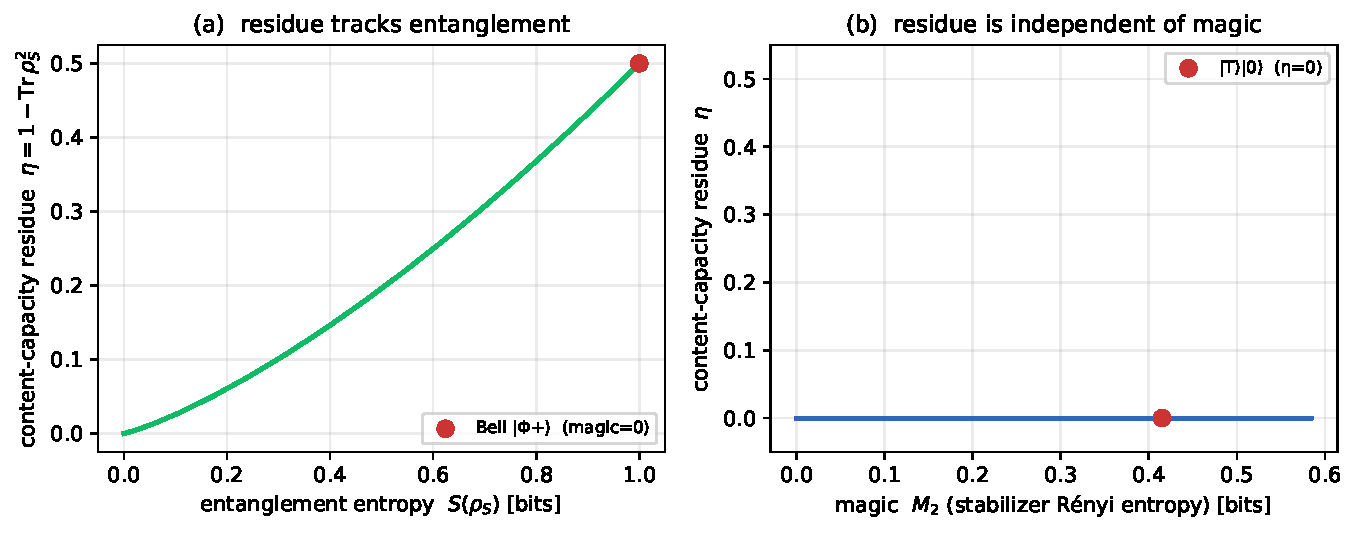
\includegraphics[width=0.92\textwidth]{figures/eta_dissociation.pdf}
\caption{\textbf{The content-capacity residue is a computable entanglement monotone, independent of
magic.} (a) Across a family of two-qubit states, the residue $\eta = 1-\mathrm{Tr}\,\rho_S^2$ rises
monotonically with the entanglement entropy of the part; the Bell state (red) realizes the maximum
\emph{at zero magic}. (b) Across a family with the part held separable, magic ($M_2$, stabilizer
R\'enyi entropy) ranges widely while $\eta$ stays identically zero; the $|T\rangle|0\rangle$ state (red)
has substantial magic and zero residue. The residue is part--whole correlation, full stop.}
\label{fig:eta}
\end{figure}

\section{The One-and-the-Many: Scale-Invariant Transactionalism}
\label{sec:many}

The one-and-the-many asks how an integrated architecture achieves global coordination (the One) without
flattening the specialized local diversity that makes its parts competent (the Many). Here the
transactional stance becomes a concrete design.

\paragraph{Rejection of the monolith.} The usual routes to global harmony are a single massive model, or
a shared universal interlingua into which every domain translates. Both destroy the Many. A universal
interlingua in particular is an epistemic trap: forcing physics, law, and biology through one common
vocabulary flattens exactly the domain-specific syntax that expertise consists in.

\paragraph{Zero-degree-of-freedom binding.} Instead, global unity is maintained as a \emph{structural
invariant} --- a binding with zero degrees of freedom (Fig.~\ref{fig:arch}). Partition the system into a
stratified hierarchy of \emph{namespaced} domain-expert nodes. Route messages \emph{deterministically by
payload type}, not through a learned (and therefore biased, and unauditable) mediator. Because routing is
type-matching, the binding layer carries no parameters to train: it cannot drift, cannot acquire a
preference, cannot become a hidden monolith. Cross-domain communication is pushed to \emph{explicit,
point-to-point typed bridges} at the domain seams, each an auditable translation between two local
vocabularies --- never a flattening into one.

\paragraph{The lazy synthesized cache.} Global consensus is never enforced as a permanent baseline. The
collective state is a \emph{lazy synthesized cache}: on a query it crystallizes \emph{locally and
on-demand} into a unified macro-state by collapsing exactly the relevant nodes; between queries the
components drift safely back into parallel superposition; and the cache self-heals at the next relevant
execution. This is the binding transaction of Sec.~\ref{sec:binding} at the architectural scale ---
which is why we call the account \emph{scale-invariant}: the same mechanism (parallel-until-measured,
unified-on-demand) resolves binding within a mind and coordination across a society of experts.
Coherence is transactional, demand-driven, and intrinsically self-balancing: you pay for the coherence
you use, when you use it, and not before.

\begin{figure}[t]
\centering
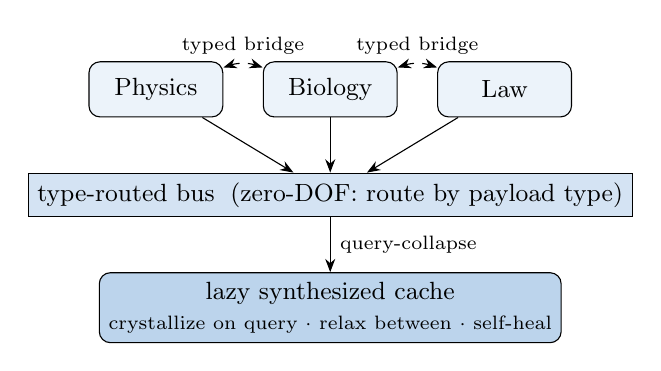
\begin{tikzpicture}[font=\small, >={Stealth[]},
  node/.style={draw, rounded corners, minimum width=1.7cm, minimum height=0.7cm, fill=accent!8},
  hub/.style={draw, fill=accent!18, minimum width=5.5cm, minimum height=0.55cm}]
  \node[node] (n1) {Physics};
  \node[node, right=0.5cm of n1] (n2) {Biology};
  \node[node, right=0.5cm of n2] (n3) {Law};
  \node[hub, below=0.7cm of n2] (bus) {type-routed bus \;(zero-DOF: route by payload type)};
  \draw[->] (n1) -- (bus); \draw[->] (n2) -- (bus); \draw[->] (n3) -- (bus);
  \draw[<->, dashed] (n1) to[bend left=18] node[above, font=\scriptsize]{typed bridge} (n2);
  \draw[<->, dashed] (n2) to[bend left=18] node[above, font=\scriptsize]{typed bridge} (n3);
  \node[draw, rounded corners, fill=accent!28, below=0.7cm of bus, minimum width=4cm, align=center] (cache) {lazy synthesized cache\\{\scriptsize crystallize on query $\cdot$ relax between $\cdot$ self-heal}};
  \draw[->] (bus) -- node[right, font=\scriptsize]{query-collapse} (cache);
\end{tikzpicture}
\caption{\textbf{The One held without flattening the Many.} Namespaced domain-expert nodes (top) keep
their local syntax. The binding bus routes deterministically by payload type and so carries zero
trainable degrees of freedom (it cannot drift into a biased monolith). Genuine cross-domain transfer
goes through explicit typed bridges at the seams. Global consensus is a lazy cache that crystallizes
on-query and relaxes between queries.}
\label{fig:arch}
\end{figure}

\section{Falsifiable Predictions}
\label{sec:pred}

Because the account is an architecture, it can be wrong in specific, checkable ways. Among its
predictions:

\begin{enumerate}\itemsep2pt
\item \textbf{Separation.} Sub-systems whose objectives operate on \emph{separate} degrees of freedom
outperform otherwise-matched systems whose objectives share degrees of freedom (destructive
interference). Falsified if shared-DOF systems perform equally.
\item \textbf{On-demand convergence.} Integrated, ``bound'' representations are present transiently
around task/query events and absent between them, rather than maintained continuously. Falsified if a
continuous global binding signal is found that is necessary for function.
\item \textbf{Per-domain memory.} A society of specialized nodes with local, per-domain memory
outperforms a monolithic shared memory of equal capacity --- with the gain non-monotonic in node
strength (mid-capacity nodes benefit most). \emph{(Independently consistent with recent results on
task-focused memorization in multimodal agents, 2026.)}
\item \textbf{No interlingua advantage.} Replacing typed point-to-point bridges with a universal
interlingua degrades cross-domain task fidelity, the loss growing with domain heterogeneity.
\item \textbf{Residue tracks correlation, not generation.} The structural correlate of an integration
event's ``richness'' (the content-capacity residue) tracks part--whole correlation, not the separate
non-stabilizer/generative resource (Fig.~\ref{fig:eta}).
\end{enumerate}

\section{Discussion}

The account is deliberately deflationary about \emph{permanence} and inflationary about \emph{events}.
It keeps the phenomena every theory must keep --- unity is real, experience is real, expertise is real
--- while denying the standing entities (the theater, the extra property, the monolith) that made them
seem mysterious. Against global-workspace theories, binding is the workspace's \emph{lighting up}, not
its continuous illumination. Against property dualism and reductive materialism alike, the hard problem
dissolves because $F_1$ and $F_2$ are parallel projections of one event, so neither the elimination of
$F_2$ nor a new law connecting it to $F_1$ is required. Against monolithic integration, the One is a
zero-DOF invariant plus a lazy cache, not a flattening.

We stress what is and is not claimed for Sec.~\ref{sec:hard}. We do not derive experience from
structure; that would re-pose the gap. We claim the demand for such a derivation mistakes a single
two-aspected event for a causal chain. Whether one finds this satisfying is partly temperamental --- but
the account earns its keep elsewhere, in Sec.~\ref{sec:many}'s buildable architecture and
Sec.~\ref{sec:pred}'s falsifiable claims, which a purely verbal dissolution cannot offer.

\section{Conclusion}

Three problems, one move: replace the standing locus of unity with the on-demand transaction. Binding
becomes the convergence event; the hard problem becomes the two aspects of that event, with felt texture
the computable residue of part--whole correlation; the one-and-the-many becomes a zero-DOF binding over
namespaced experts with a lazy synthesized cache. The wager of this paper is that these are not
positions to be defended but systems to be built --- and that a mind so built will exhibit the
predictions of Sec.~\ref{sec:pred}. The mysticism was vestigial. What remains is architecture.

\appendix
\section{The residue computation}
Figure~\ref{fig:eta} is generated by \texttt{figures/make\_eta\_figure.py}. For a pure two-qubit state
$|\psi\rangle$ with subsystem $S$, $\eta(S)=1-\mathrm{Tr}\,\rho_S^2$ where $\rho_S=\mathrm{Tr}_E
|\psi\rangle\langle\psi|$. Magic is the stabilizer 2-R\'enyi entropy $M_2=-\log_2\!\big(d\sum_P
\Xi_P^2\big)$ with $\Xi_P=\langle\psi|P|\psi\rangle^2/d$ over all Pauli strings $P$ and $d=2^n$. The
double dissociation (Bell: $\eta=0.5,\,M_2=0$; $|T\rangle|0\rangle$: $\eta=0,\,M_2=0.415$) establishes
that $\eta$ is an entanglement monotone independent of magic.

\end{document}
